\documentclass[11pt]{article}
\usepackage[margin=2.2cm]{geometry}
\usepackage{amsmath,amssymb}
\usepackage[most]{tcolorbox}
\usepackage{xcolor}
\usepackage{tikz}
\usetikzlibrary{arrows.meta,positioning,calc}
\usepackage{booktabs}

\definecolor{stageblue}{RGB}{31,119,180}
\definecolor{stagegreen}{RGB}{44,160,44}
\definecolor{chanred}{RGB}{214,39,40}

\title{\textbf{Chained NPD for Memory MAC}\\[5pt]
\large The Math on the Board}
\author{}
\date{}

\begin{document}
\maketitle
\thispagestyle{empty}

%% ============================================================
\section{The Chained Decoding Idea}

Two users $U$ and $V$ transmit through a shared channel. At the \textbf{corner rate} (Class~C path), we decode in two stages:

\begin{tcolorbox}[colback=blue!5,colframe=stageblue,title=Stage 1: Decode $U$ (treat $V$ as noise)]
\[
\hat{u}_i = \arg\max_{u_i \in \{0,1\}} \; P(u_i \mid z_1^N,\, \hat{u}_1^{i-1})
\]
$V$ is unknown $\Rightarrow$ marginalized as uniform noise. This is a \textbf{single-user} decoding problem on the effective channel $P(Z \mid X) = \sum_Y P(Y) \cdot P(Z \mid X, Y)$.
\end{tcolorbox}

\begin{tcolorbox}[colback=green!5,colframe=stagegreen,title=Stage 2: Decode $V$ given $\hat{U}$]
\[
\hat{v}_i = \arg\max_{v_i \in \{0,1\}} \; P(v_i \mid z_1^N,\, \hat{u}_1^N,\, \hat{v}_1^{i-1})
\]
$\hat{U}$ is known from Stage~1 $\Rightarrow$ this is also a single-user problem, on the effective channel $P(Z \mid Y, \hat{X})$.
\end{tcolorbox}

\medskip
Each stage produces a \textbf{binary LLR} at each position:
\[
\text{LLR}_i = \log \frac{P(\text{bit}_i = 0 \mid \text{observations})}{P(\text{bit}_i = 1 \mid \text{observations})}
\]

%% ============================================================
\section{Architecture: What Changes Per Channel}

\begin{center}
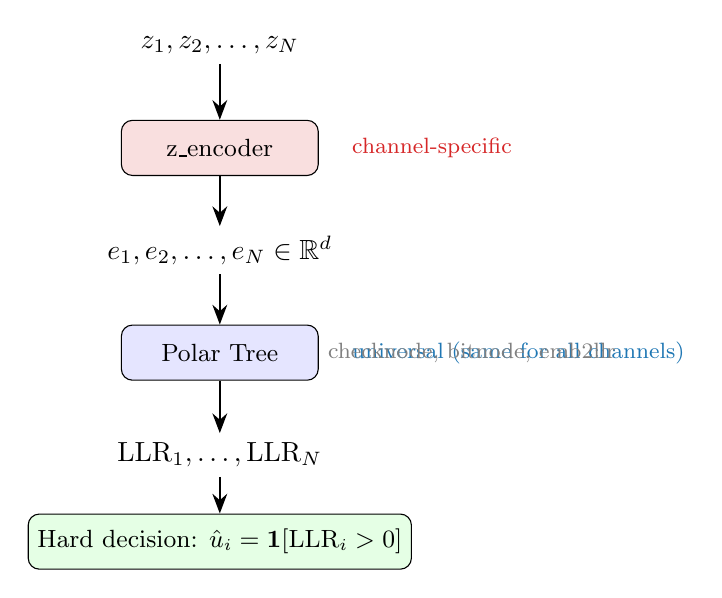
\begin{tikzpicture}[
    box/.style={draw, rounded corners, minimum width=2.5cm, minimum height=0.7cm, align=center, font=\small},
    arrow/.style={-{Stealth[length=2.5mm]}, thick}
]
% z input
\node (z) at (0,0) {$z_1, z_2, \ldots, z_N$};

% z_encoder
\node[box, fill=chanred!15] (zenc) at (0,-1.3) {z\_encoder};
\node[right=0.3cm of zenc, font=\footnotesize, text=chanred] {channel-specific};

% embeddings
\node (emb) at (0,-2.6) {$e_1, e_2, \ldots, e_N \in \mathbb{R}^d$};

% tree
\node[box, fill=blue!10] (tree) at (0,-3.9) {Polar Tree};
\node[right=0.3cm of tree, font=\footnotesize, text=stageblue] {universal (same for all channels)};

% tree ops
\node[font=\footnotesize, text=gray] at (3.2,-3.9) {checknode, bitnode, emb2llr};

% LLR
\node (llr) at (0,-5.2) {$\text{LLR}_1, \ldots, \text{LLR}_N$};

% decisions
\node[box, fill=green!10] (dec) at (0,-6.3) {Hard decision: $\hat{u}_i = \mathbf{1}[\text{LLR}_i > 0]$};

\draw[arrow] (z) -- (zenc);
\draw[arrow] (zenc) -- (emb);
\draw[arrow] (emb) -- (tree);
\draw[arrow] (tree) -- (llr);
\draw[arrow] (llr) -- (dec);
\end{tikzpicture}
\end{center}

\medskip
\textbf{Key insight:} Only the z\_encoder changes between channels. The tree operations are \textbf{identical}.

%% ============================================================
\section{The Three Channels}

\subsection{GMAC (Memoryless)}

\[
\boxed{Z_i = (1-2X_i) + (1-2Y_i) + W_i, \quad W_i \sim \mathcal{N}(0, \sigma^2)}
\]

\begin{itemize}
\item Each $Z_i$ depends only on $(X_i, Y_i)$ --- no memory.
\item \textbf{z\_encoder:} pointwise MLP. $\; e_i = \text{MLP}(z_i)$. Each position processed independently.
\item \textbf{Stage 1 effective channel:} $P(Z_i \mid X_i) = \frac{1}{2}\bigl[\mathcal{N}(Z_i;\, s_{X_i}{+}1,\, \sigma^2) + \mathcal{N}(Z_i;\, s_{X_i}{-}1,\, \sigma^2)\bigr]$

where $s_{X_i} = 1 - 2X_i$. This is a Gaussian \textbf{mixture} (marginalize $Y_i$ uniform).
\end{itemize}

\subsection{ISI-MAC (Finite-State Memory)}

\[
\boxed{Z_i = (1{-}2X_i) + (1{-}2Y_i) + h\bigl((1{-}2X_{i-1}) + (1{-}2Y_{i-1})\bigr) + W_i}
\]

\begin{itemize}
\item $Z_i$ depends on \textbf{current and previous} inputs. Parameter $h = 0.3$.
\item State: $S_i = (X_{i-1}, Y_{i-1}) \in \{0,1\}^2$ --- 4 states.
\item \textbf{z\_encoder:} Bidirectional GRU over the full sequence.
\[
(e_1, \ldots, e_N) = \text{BiGRU}(z_1, \ldots, z_N)
\]
The BiGRU sees neighboring $z$ values and learns to cancel the ISI interference.
\item \textbf{Stage 1 effective channel:} $P(Z_i \mid X_i, S_i) = \frac{1}{2}\sum_{Y_i} P(Z_i \mid X_i, Y_i, S_i)$

This is a finite-state channel $\Rightarrow$ trellis SC decoder exists (our analytical baseline).
\end{itemize}

\subsection{MA-AGN MAC (Continuous-State Memory)}

\[
\boxed{Z_i = (1{-}2X_i) + (1{-}2Y_i) + N_i, \quad N_i = \alpha \cdot N_{i-1} + W_i}
\]

\begin{itemize}
\item Noise $N_i$ is an AR(1) process with parameter $\alpha$. Noise samples are \textbf{correlated}.
\item State: $N_{i-1} \in \mathbb{R}$ --- \textbf{continuous}, not finite.
\item \textbf{z\_encoder:} Same BiGRU. Learns to exploit the noise correlation.
\item \textbf{Stage 1 effective channel:} No closed-form trellis (continuous state).
\[
P(Z_i \mid X_i, N_{i-1}) = \frac{1}{2}\sum_{Y_i} \mathcal{N}\bigl(Z_i;\, s_{X_i} + s_{Y_i} + \alpha N_{i-1},\;\sigma^2(1-\alpha^2)\bigr)
\]
\textbf{No analytical decoder exists} $\Rightarrow$ neural decoder is the only option.
\end{itemize}

%% ============================================================
\section{Training: fast\_ce (Parallel)}

Each stage is trained with \textbf{fast\_ce}: teacher-forced binary cross-entropy at every tree depth simultaneously.

\begin{enumerate}
\item Generate codewords: $u \to x = \text{polar\_encode}(u)$, same for $v \to y$.
\item Channel: $z = \text{channel}(x, y)$.
\item z\_encoder: $e = \text{z\_enc}(z)$ (pointwise or BiGRU).
\item At each tree depth $\ell = 0, 1, \ldots, \log_2 N$:
\begin{itemize}
\item Apply checknode/bitnode using \textbf{true codeword bits} (teacher forcing).
\item Compute $\text{LLR} = \text{emb2llr}(e)$ at all positions.
\item Loss: $\text{BCE}(\text{LLR}, \text{true bits})$.
\end{itemize}
\item Total loss = average over all depths. One backward pass.
\end{enumerate}

\textbf{Gradient depth:} $O(\log N)$ instead of $O(N \log N)$ for sequential training.

%% ============================================================
\section{Summary Table}

\renewcommand{\arraystretch}{1.3}
\begin{center}\small
\begin{tabular}{@{}l c c c c@{}}
\toprule
& \textbf{GMAC} & \textbf{ISI-MAC} & \textbf{MA-AGN} \\
\midrule
Memory & None & Finite ($|S|=4$) & Continuous ($S \in \mathbb{R}$) \\
z\_encoder & Pointwise MLP & BiGRU & BiGRU \\
Analytical SC & Yes (exact) & Yes (trellis) & \textbf{No} \\
Tree ops & \multicolumn{3}{c}{Same MLPs for all channels} \\
Training & \multicolumn{3}{c}{fast\_ce, $O(\log N)$ gradient depth} \\
\midrule
NPD beats SC? & $N \le 64$ & $N \le 64$ & $N \le 64$ ($\alpha{=}0.9$) \\
Wall at & $N = 128^\dagger$ & $N = 512$ & $N = 128$ \\
\bottomrule
\end{tabular}
\end{center}

{\footnotesize $^\dagger$GMAC C wall at $N=128$ is due to missing 3-phase frozen-set design, not decoder limitation.}

%% ============================================================
\newpage
\section{Worked Example: GMAC Chained SC at $N=2$}

\textbf{Setup:} $u = (0,1)$, $v = (1,0)$. Encoding: $x = (1,1)$, $y = (1,0)$.\\
Received: $z_1 = -1.75$, $z_2 = -0.15$. SNR = 6\,dB ($\sigma^2 = 0.251$).

\subsection*{Stage 1: Decode $U$ (marginalize $V$ as uniform)}

Effective single-user channel: $P(z_i \mid x_i) = \tfrac{1}{2}[P(z_i \mid x_i, y{=}0) + P(z_i \mid x_i, y{=}1)]$:

\[
P(z_1 \mid x{=}0) = 0.0009, \quad P(z_1 \mid x{=}1) = 0.3524
\]
\[
P(z_2 \mid x{=}0) = 0.3807, \quad P(z_2 \mid x{=}1) = 0.3811
\]

Effective LLRs:
\[
\text{LLR}_{z_1} = \log\frac{0.0009}{0.3524} = -5.98, \qquad
\text{LLR}_{z_2} = \log\frac{0.3807}{0.3811} = -0.001
\]

$z_1$ strongly says $x_1 = 1$. $z_2$ is ambiguous (the (0,1)/(1,0) collision at $z \approx 0$).

\medskip
\textbf{CalcLeft} (f-function, decode $u_1$):
\[
\text{LLR}_{u_1} = 2\tanh^{-1}\!\bigl(\tanh(\tfrac{-5.98}{2}) \cdot \tanh(\tfrac{-0.001}{2})\bigr) = +0.001
\]
$\hat{u}_1 = 0$ \; (barely, LLR $\approx$ 0). \textbf{Correct} ($u_1 = 0$).

\medskip
\textbf{CalcRight} (g-function, decode $u_2$):
\[
\text{LLR}_{u_2} = \text{LLR}_{z_2} + (1 - 2\hat{u}_1) \cdot \text{LLR}_{z_1} = -0.001 + 1 \times (-5.98) = -5.98
\]
$\hat{u}_2 = 1$ \; (strong). \textbf{Correct} ($u_2 = 1$).

\subsection*{Stage 2: Decode $V$ given $\hat{U} = (0,1)$}

Now $X$ is known: $\hat{x}_1 = \hat{u}_1 \oplus \hat{u}_2 = 1$, $\hat{x}_2 = \hat{u}_2 = 1$. BPSK: $s_{\hat{x}} = (-1, -1)$.

Clean single-user channel: $P(z_i \mid y_i, \hat{x}_i) = \mathcal{N}(z_i;\, s_{\hat{x}_i} + s_{y_i},\, \sigma^2)$:
\[
\text{LLR}_{z_1}^{(v)} = \log\frac{\mathcal{N}(-1.75;\, 0,\, \sigma^2)}{\mathcal{N}(-1.75;\, -2,\, \sigma^2)} = \log\frac{0.0018}{0.7031} = -5.98
\]
\[
\text{LLR}_{z_2}^{(v)} = \log\frac{\mathcal{N}(-0.15;\, 0,\, \sigma^2)}{\mathcal{N}(-0.15;\, -2,\, \sigma^2)} = \log\frac{0.7614}{0.0009} = +6.77
\]

\textbf{CalcLeft:} $\text{LLR}_{v_1} = 2\tanh^{-1}\!\bigl(\tanh(\tfrac{-5.98}{2})\cdot\tanh(\tfrac{6.77}{2})\bigr) = -5.60$. \; $\hat{v}_1 = 1$. \textbf{Correct.}

\textbf{CalcRight:} $\text{LLR}_{v_2} = 6.77 + (1-2\cdot 1)\cdot(-5.98) = +12.75$. \; $\hat{v}_2 = 0$. \textbf{Correct.}

\subsection*{Key Observations}

\begin{enumerate}[nosep]
\item \textbf{Stage 1 is harder:} $z_2$ gives LLR $\approx 0$ because $P(z|x{=}0)$ and $P(z|x{=}1)$ are nearly equal after marginalizing $V$. The Gaussian mixture from $V$-marginalization creates an information ``dead zone'' near $z = 0$.
\item \textbf{Stage 2 is easier:} once $X$ is known, each $z_i$ gives a clean Gaussian LLR (no mixture). Stage~2 LLRs ($\pm$5.98, $\pm$6.77) are much stronger than Stage~1.
\item \textbf{Chaining works:} even though Stage~1 barely resolves $u_1$, the cascading through CalcRight recovers $u_2$ strongly, and Stage~2 decodes $V$ cleanly.
\end{enumerate}

\end{document}
